\documentclass[twoside]{book}

% Packages required by doxygen
\usepackage{fixltx2e}
\usepackage{calc}
\usepackage{doxygen}
\usepackage[export]{adjustbox} % also loads graphicx
\usepackage{graphicx}
\usepackage[utf8]{inputenc}
\usepackage{makeidx}
\usepackage{multicol}
\usepackage{multirow}
\PassOptionsToPackage{warn}{textcomp}
\usepackage{textcomp}
\usepackage[nointegrals]{wasysym}
\usepackage[table]{xcolor}

% Font selection
\usepackage[T1]{fontenc}
\usepackage[scaled=.90]{helvet}
\usepackage{courier}
\usepackage{amssymb}
\usepackage{sectsty}
\renewcommand{\familydefault}{\sfdefault}
\allsectionsfont{%
  \fontseries{bc}\selectfont%
  \color{darkgray}%
}
\renewcommand{\DoxyLabelFont}{%
  \fontseries{bc}\selectfont%
  \color{darkgray}%
}
\newcommand{\+}{\discretionary{\mbox{\scriptsize$\hookleftarrow$}}{}{}}

% Page & text layout
\usepackage{geometry}
\geometry{%
  a4paper,%
  top=2.5cm,%
  bottom=2.5cm,%
  left=2.5cm,%
  right=2.5cm%
}
\tolerance=750
\hfuzz=15pt
\hbadness=750
\setlength{\emergencystretch}{15pt}
\setlength{\parindent}{0cm}
\setlength{\parskip}{3ex plus 2ex minus 2ex}
\makeatletter
\renewcommand{\paragraph}{%
  \@startsection{paragraph}{4}{0ex}{-1.0ex}{1.0ex}{%
    \normalfont\normalsize\bfseries\SS@parafont%
  }%
}
\renewcommand{\subparagraph}{%
  \@startsection{subparagraph}{5}{0ex}{-1.0ex}{1.0ex}{%
    \normalfont\normalsize\bfseries\SS@subparafont%
  }%
}
\makeatother

% Headers & footers
\usepackage{fancyhdr}
\pagestyle{fancyplain}
\fancyhead[LE]{\fancyplain{}{\bfseries\thepage}}
\fancyhead[CE]{\fancyplain{}{}}
\fancyhead[RE]{\fancyplain{}{\bfseries\leftmark}}
\fancyhead[LO]{\fancyplain{}{\bfseries\rightmark}}
\fancyhead[CO]{\fancyplain{}{}}
\fancyhead[RO]{\fancyplain{}{\bfseries\thepage}}
\fancyfoot[LE]{\fancyplain{}{}}
\fancyfoot[CE]{\fancyplain{}{}}
\fancyfoot[RE]{\fancyplain{}{\bfseries\scriptsize Generated by Doxygen }}
\fancyfoot[LO]{\fancyplain{}{\bfseries\scriptsize Generated by Doxygen }}
\fancyfoot[CO]{\fancyplain{}{}}
\fancyfoot[RO]{\fancyplain{}{}}
\renewcommand{\footrulewidth}{0.4pt}
\renewcommand{\chaptermark}[1]{%
  \markboth{#1}{}%
}
\renewcommand{\sectionmark}[1]{%
  \markright{\thesection\ #1}%
}

% Indices & bibliography
\usepackage{natbib}
\usepackage[titles]{tocloft}
\setcounter{tocdepth}{3}
\setcounter{secnumdepth}{5}
\makeindex

% Hyperlinks (required, but should be loaded last)
\usepackage{ifpdf}
\ifpdf
  \usepackage[pdftex,pagebackref=true]{hyperref}
\else
  \usepackage[ps2pdf,pagebackref=true]{hyperref}
\fi
\hypersetup{%
  colorlinks=true,%
  linkcolor=blue,%
  citecolor=blue,%
  unicode%
}

% Custom commands
\newcommand{\clearemptydoublepage}{%
  \newpage{\pagestyle{empty}\cleardoublepage}%
}

\usepackage{caption}
\captionsetup{labelsep=space,justification=centering,font={bf},singlelinecheck=off,skip=4pt,position=top}

%===== C O N T E N T S =====

\begin{document}

% Titlepage & ToC
\hypersetup{pageanchor=false,
             bookmarksnumbered=true,
             pdfencoding=unicode
            }
\pagenumbering{alph}
\begin{titlepage}
\vspace*{7cm}
\begin{center}%
{\Large Sourlib-\/bbn }\\
\vspace*{1cm}
{\large Generated by Doxygen 1.8.13}\\
\end{center}
\end{titlepage}
\clearemptydoublepage
\pagenumbering{roman}
\tableofcontents
\clearemptydoublepage
\pagenumbering{arabic}
\hypersetup{pageanchor=true}

%--- Begin generated contents ---
\chapter{Sourbbn-\/lib\+: C++ Library for solving Second Order Uncertainy in Bayesian Belief Networks}
\label{index}\hypertarget{index}{}Bayesian Belief Networks (B\+B\+Ns) are a type of probabilistic graphical model where the joint distribution over all variables in the model is represented by directed acyclic graph. Nodes in the graph represent the probability distribution of a given variable conditional on it\textquotesingle{}s parents in the graph. These conditional distributions are stored as conditional probability tables. The values in conditional probability tables are often inferred from data and are not known exactly. This library provides a set of C/\+C++ classes and functions implementing the Mean\+Var and Buck\+Elim+ algorithms, extracted from \href{https://doi.org/10.1016/j.artint.2007.09.004}{\tt Van Allen et al. 2008}, for querying B\+B\+Ns with uncertain data. 
\chapter{Class Index}
\section{Class List}
Here are the classes, structs, unions and interfaces with brief descriptions\+:\begin{DoxyCompactList}
\item\contentsline{section}{\hyperlink{structsourbbn_1_1Bucket}{sourbbn\+::\+Bucket} }{\pageref{structsourbbn_1_1Bucket}}{}
\item\contentsline{section}{\hyperlink{structsourbbn_1_1BucketList}{sourbbn\+::\+Bucket\+List} }{\pageref{structsourbbn_1_1BucketList}}{}
\item\contentsline{section}{\hyperlink{structsourbbn_1_1CPTable}{sourbbn\+::\+C\+P\+Table} }{\pageref{structsourbbn_1_1CPTable}}{}
\item\contentsline{section}{\hyperlink{classsourbbn_1_1FieldSchema}{sourbbn\+::\+Field\+Schema} }{\pageref{classsourbbn_1_1FieldSchema}}{}
\item\contentsline{section}{\hyperlink{unionsourbbn_1_1FieldValue}{sourbbn\+::\+Field\+Value} }{\pageref{unionsourbbn_1_1FieldValue}}{}
\item\contentsline{section}{\hyperlink{classsourbbn_1_1RowSchema}{sourbbn\+::\+Row\+Schema} }{\pageref{classsourbbn_1_1RowSchema}}{}
\item\contentsline{section}{\hyperlink{classsourbbn_1_1RowValue}{sourbbn\+::\+Row\+Value} }{\pageref{classsourbbn_1_1RowValue}}{}
\item\contentsline{section}{\hyperlink{classsourbbn_1_1Sourbbn}{sourbbn\+::\+Sourbbn} }{\pageref{classsourbbn_1_1Sourbbn}}{}
\item\contentsline{section}{\hyperlink{classsourbbn_1_1Sourbbn_1_1sourbbn__impl}{sourbbn\+::\+Sourbbn\+::sourbbn\+\_\+impl} }{\pageref{classsourbbn_1_1Sourbbn_1_1sourbbn__impl}}{}
\end{DoxyCompactList}

\chapter{Class Documentation}
\hypertarget{structsourbbn_1_1Bucket}{}\section{sourbbn\+:\+:Bucket Struct Reference}
\label{structsourbbn_1_1Bucket}\index{sourbbn\+::\+Bucket@{sourbbn\+::\+Bucket}}
\subsection*{Public Member Functions}
\begin{DoxyCompactItemize}
\item 
\mbox{\Hypertarget{structsourbbn_1_1Bucket_a632c74de8383ee2e2c26fab02a5962ba}\label{structsourbbn_1_1Bucket_a632c74de8383ee2e2c26fab02a5962ba}} 
{\bfseries Bucket} (std\+::string \&bid)
\item 
\mbox{\Hypertarget{structsourbbn_1_1Bucket_a61973d198869d9d1fd7f5dcfcc342cae}\label{structsourbbn_1_1Bucket_a61973d198869d9d1fd7f5dcfcc342cae}} 
{\bfseries Bucket} (std\+::string \&\&bid)
\item 
\mbox{\Hypertarget{structsourbbn_1_1Bucket_ab07b7b82324f59048ddb2fa6c79b410b}\label{structsourbbn_1_1Bucket_ab07b7b82324f59048ddb2fa6c79b410b}} 
{\bfseries Bucket} (std\+::string \&bid, \hyperlink{structsourbbn_1_1CPTable}{C\+P\+Table} \&b\+\_\+tbl)
\item 
\mbox{\Hypertarget{structsourbbn_1_1Bucket_a9361e6faa526a48ed3b81a7da57976da}\label{structsourbbn_1_1Bucket_a9361e6faa526a48ed3b81a7da57976da}} 
{\bfseries Bucket} (std\+::string \&\&bid, \hyperlink{structsourbbn_1_1CPTable}{C\+P\+Table} \&b\+\_\+tbl)
\item 
\mbox{\Hypertarget{structsourbbn_1_1Bucket_a2b553ba424d4eddd8ce9921be7c62e49}\label{structsourbbn_1_1Bucket_a2b553ba424d4eddd8ce9921be7c62e49}} 
{\bfseries Bucket} (std\+::string \&bid, std\+::vector$<$ \hyperlink{structsourbbn_1_1CPTable}{C\+P\+Table} $>$ \&b\+\_\+tbls)
\item 
\mbox{\Hypertarget{structsourbbn_1_1Bucket_ad511cda44fb03dfc6d989be8dc6af10c}\label{structsourbbn_1_1Bucket_ad511cda44fb03dfc6d989be8dc6af10c}} 
{\bfseries Bucket} (std\+::string \&\&bid, std\+::vector$<$ \hyperlink{structsourbbn_1_1CPTable}{C\+P\+Table} $>$ \&b\+\_\+tbls)
\item 
\mbox{\Hypertarget{structsourbbn_1_1Bucket_a1d13ee3e3b92f331471a8c4802c827c8}\label{structsourbbn_1_1Bucket_a1d13ee3e3b92f331471a8c4802c827c8}} 
{\bfseries Bucket} (std\+::string \&\&bid, std\+::vector$<$ \hyperlink{structsourbbn_1_1CPTable}{C\+P\+Table} $>$ \&\&b\+\_\+tbls)
\item 
\mbox{\Hypertarget{structsourbbn_1_1Bucket_a8efe97b92bf7bbe679c112bb178d4ce2}\label{structsourbbn_1_1Bucket_a8efe97b92bf7bbe679c112bb178d4ce2}} 
void {\bfseries append} (\hyperlink{structsourbbn_1_1CPTable}{C\+P\+Table} \&b\+\_\+tbl)
\end{DoxyCompactItemize}
\subsection*{Public Attributes}
\begin{DoxyCompactItemize}
\item 
\mbox{\Hypertarget{structsourbbn_1_1Bucket_a8fc740fec9c981b4ec5f1f7cfdad583b}\label{structsourbbn_1_1Bucket_a8fc740fec9c981b4ec5f1f7cfdad583b}} 
std\+::string {\bfseries bucket\+\_\+id}
\item 
\mbox{\Hypertarget{structsourbbn_1_1Bucket_afd1f29b2aa4d81d7af0cb635c6b17366}\label{structsourbbn_1_1Bucket_afd1f29b2aa4d81d7af0cb635c6b17366}} 
std\+::vector$<$ \hyperlink{structsourbbn_1_1CPTable}{C\+P\+Table} $>$ {\bfseries bucket\+\_\+tables}
\end{DoxyCompactItemize}


\subsection{Detailed Description}


Definition at line 30 of file buckets.\+hpp.



The documentation for this struct was generated from the following files\+:\begin{DoxyCompactItemize}
\item 
include/sourbbn/buckets.\+hpp\item 
src/buckets.\+cpp\end{DoxyCompactItemize}

\hypertarget{structsourbbn_1_1BucketList}{}\section{sourbbn\+:\+:Bucket\+List Struct Reference}
\label{structsourbbn_1_1BucketList}\index{sourbbn\+::\+Bucket\+List@{sourbbn\+::\+Bucket\+List}}
\subsection*{Public Member Functions}
\begin{DoxyCompactItemize}
\item 
\mbox{\Hypertarget{structsourbbn_1_1BucketList_aff121e1039b574c61b94e299653fee03}\label{structsourbbn_1_1BucketList_aff121e1039b574c61b94e299653fee03}} 
{\bfseries Bucket\+List} (std\+::vector$<$ std\+::string $>$ \&pi)
\item 
\mbox{\Hypertarget{structsourbbn_1_1BucketList_ae67265af182b411ef3d9c63d14534a80}\label{structsourbbn_1_1BucketList_ae67265af182b411ef3d9c63d14534a80}} 
float {\bfseries Buck\+Elim} ()
\end{DoxyCompactItemize}
\subsection*{Public Attributes}
\begin{DoxyCompactItemize}
\item 
\mbox{\Hypertarget{structsourbbn_1_1BucketList_ae7f9bad12a59676dfc1693b1f30d3f26}\label{structsourbbn_1_1BucketList_ae7f9bad12a59676dfc1693b1f30d3f26}} 
std\+::vector$<$ std\+::string $>$ {\bfseries variable\+\_\+order\+\_\+pi}
\item 
\mbox{\Hypertarget{structsourbbn_1_1BucketList_af141e28b4e77be7f659e257af006c1f3}\label{structsourbbn_1_1BucketList_af141e28b4e77be7f659e257af006c1f3}} 
std\+::unordered\+\_\+map$<$ std\+::string, \hyperlink{structsourbbn_1_1Bucket}{Bucket} $>$ {\bfseries buckets}
\end{DoxyCompactItemize}


\subsection{Detailed Description}


Definition at line 48 of file buckets.\+hpp.



The documentation for this struct was generated from the following files\+:\begin{DoxyCompactItemize}
\item 
include/sourbbn/buckets.\+hpp\item 
src/buckets.\+cpp\end{DoxyCompactItemize}

\hypertarget{structsourbbn_1_1CPTable}{}\section{sourbbn\+:\+:C\+P\+Table Struct Reference}
\label{structsourbbn_1_1CPTable}\index{sourbbn\+::\+C\+P\+Table@{sourbbn\+::\+C\+P\+Table}}


Collaboration diagram for sourbbn\+:\+:C\+P\+Table\+:
\nopagebreak
\begin{figure}[H]
\begin{center}
\leavevmode
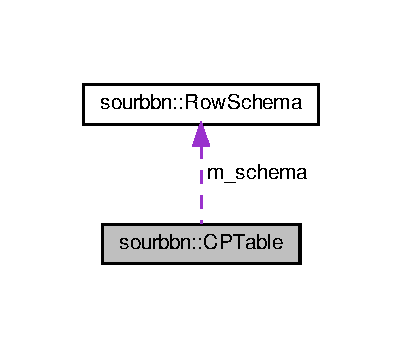
\includegraphics[width=193pt]{structsourbbn_1_1CPTable__coll__graph}
\end{center}
\end{figure}
\subsection*{Public Member Functions}
\begin{DoxyCompactItemize}
\item 
\mbox{\Hypertarget{structsourbbn_1_1CPTable_a91772bb85dc0edfb3c659730fb1570f8}\label{structsourbbn_1_1CPTable_a91772bb85dc0edfb3c659730fb1570f8}} 
{\bfseries C\+P\+Table} (const \hyperlink{classsourbbn_1_1RowSchema}{Row\+Schema} \&ms)
\item 
\mbox{\Hypertarget{structsourbbn_1_1CPTable_a397df7e9d67d895ada6d8c1c99736d3c}\label{structsourbbn_1_1CPTable_a397df7e9d67d895ada6d8c1c99736d3c}} 
{\bfseries C\+P\+Table} (const \hyperlink{structsourbbn_1_1CPTable}{C\+P\+Table} \&other\+\_\+table)
\item 
\mbox{\Hypertarget{structsourbbn_1_1CPTable_a2951c4f0b57373b338e0a5859f730d9c}\label{structsourbbn_1_1CPTable_a2951c4f0b57373b338e0a5859f730d9c}} 
{\bfseries C\+P\+Table} (\hyperlink{structsourbbn_1_1CPTable}{C\+P\+Table} \&\&other\+\_\+table) noexcept
\item 
\mbox{\Hypertarget{structsourbbn_1_1CPTable_a7ecc27010fb8e1754a9b82c3d760790e}\label{structsourbbn_1_1CPTable_a7ecc27010fb8e1754a9b82c3d760790e}} 
\hyperlink{structsourbbn_1_1CPTable}{C\+P\+Table} \& {\bfseries operator=} (const \hyperlink{structsourbbn_1_1CPTable}{C\+P\+Table} \&other\+\_\+table)
\item 
\mbox{\Hypertarget{structsourbbn_1_1CPTable_a40b09f0f86067fd7cccefae925012ee5}\label{structsourbbn_1_1CPTable_a40b09f0f86067fd7cccefae925012ee5}} 
\hyperlink{structsourbbn_1_1CPTable}{C\+P\+Table} \& {\bfseries operator=} (\hyperlink{structsourbbn_1_1CPTable}{C\+P\+Table} \&\&other\+\_\+table) noexcept
\item 
\mbox{\Hypertarget{structsourbbn_1_1CPTable_aff3f0def2ea100b7468709e0e0b69f41}\label{structsourbbn_1_1CPTable_aff3f0def2ea100b7468709e0e0b69f41}} 
\hyperlink{classsourbbn_1_1RowSchema}{Row\+Schema} {\bfseries scheme} ()
\item 
\mbox{\Hypertarget{structsourbbn_1_1CPTable_aea66324ae4cb8f0b6ae2d847a1832c7f}\label{structsourbbn_1_1CPTable_aea66324ae4cb8f0b6ae2d847a1832c7f}} 
float {\bfseries column\+\_\+sum} (const std\+::string \&var)
\end{DoxyCompactItemize}
\subsection*{Static Public Member Functions}
\begin{DoxyCompactItemize}
\item 
\mbox{\Hypertarget{structsourbbn_1_1CPTable_a8b9a998b6c9f03e035a16b8b300a1f93}\label{structsourbbn_1_1CPTable_a8b9a998b6c9f03e035a16b8b300a1f93}} 
static int {\bfseries schema\+\_\+callback} (void $\ast$data, int argc, char $\ast$$\ast$argv, char $\ast$$\ast$az\+Col\+Name)
\item 
\mbox{\Hypertarget{structsourbbn_1_1CPTable_abcfc4ec8b891c9c4bae1d8d1ca85d528}\label{structsourbbn_1_1CPTable_abcfc4ec8b891c9c4bae1d8d1ca85d528}} 
static int {\bfseries data\+\_\+callback} (void $\ast$data, int argc, char $\ast$$\ast$argv, char $\ast$$\ast$az\+Col\+Name)
\end{DoxyCompactItemize}
\subsection*{Public Attributes}
\begin{DoxyCompactItemize}
\item 
\mbox{\Hypertarget{structsourbbn_1_1CPTable_ae0601adf81fe798848d3a39a21945a26}\label{structsourbbn_1_1CPTable_ae0601adf81fe798848d3a39a21945a26}} 
\hyperlink{classsourbbn_1_1RowSchema}{Row\+Schema} {\bfseries m\+\_\+schema}
\item 
\mbox{\Hypertarget{structsourbbn_1_1CPTable_aa9ba48439d7b426f69530d383a9f53f8}\label{structsourbbn_1_1CPTable_aa9ba48439d7b426f69530d383a9f53f8}} 
std\+::vector$<$ \hyperlink{classsourbbn_1_1RowValue}{Row\+Value} $>$ {\bfseries m\+\_\+rows}
\item 
\mbox{\Hypertarget{structsourbbn_1_1CPTable_a2bdd82dafd989d93b49a94f599782d16}\label{structsourbbn_1_1CPTable_a2bdd82dafd989d93b49a94f599782d16}} 
std\+::string {\bfseries table\+\_\+name}
\item 
\mbox{\Hypertarget{structsourbbn_1_1CPTable_a1712ff346b06c75056f6736633042551}\label{structsourbbn_1_1CPTable_a1712ff346b06c75056f6736633042551}} 
const std\+::unordered\+\_\+map$<$ std\+::string, int $>$ {\bfseries protected\+\_\+names} = \{\{\char`\"{}p\char`\"{},1\},\{\char`\"{}m\char`\"{},1\},\{\char`\"{}dist\char`\"{},1\}\}
\end{DoxyCompactItemize}


\subsection{Detailed Description}


Definition at line 90 of file cptable.\+hpp.



The documentation for this struct was generated from the following files\+:\begin{DoxyCompactItemize}
\item 
include/sourbbn/cptable.\+hpp\item 
src/cptable.\+cpp\end{DoxyCompactItemize}

\hypertarget{classsourbbn_1_1FieldSchema}{}\section{sourbbn\+:\+:Field\+Schema Class Reference}
\label{classsourbbn_1_1FieldSchema}\index{sourbbn\+::\+Field\+Schema@{sourbbn\+::\+Field\+Schema}}
\subsection*{Public Member Functions}
\begin{DoxyCompactItemize}
\item 
\mbox{\Hypertarget{classsourbbn_1_1FieldSchema_a18964de27fa3ed6e1609af7f1762c5d2}\label{classsourbbn_1_1FieldSchema_a18964de27fa3ed6e1609af7f1762c5d2}} 
{\bfseries Field\+Schema} (Field\+Type mt, std\+::string mn)
\item 
\mbox{\Hypertarget{classsourbbn_1_1FieldSchema_aebe466cbf3b8435f662aa5d20f1c920e}\label{classsourbbn_1_1FieldSchema_aebe466cbf3b8435f662aa5d20f1c920e}} 
std\+::string {\bfseries get\+\_\+name} () const
\item 
\mbox{\Hypertarget{classsourbbn_1_1FieldSchema_a3b6c653ab6409221f757e56e1df10c9e}\label{classsourbbn_1_1FieldSchema_a3b6c653ab6409221f757e56e1df10c9e}} 
Field\+Type {\bfseries get\+\_\+type} () const
\item 
\mbox{\Hypertarget{classsourbbn_1_1FieldSchema_a9c0632a1857f34907bdc95338dca1589}\label{classsourbbn_1_1FieldSchema_a9c0632a1857f34907bdc95338dca1589}} 
bool {\bfseries operator==} (const \hyperlink{classsourbbn_1_1FieldSchema}{Field\+Schema} \&other) const
\item 
\mbox{\Hypertarget{classsourbbn_1_1FieldSchema_a2fe79d2a7f8d8c8bbbbfac798f396301}\label{classsourbbn_1_1FieldSchema_a2fe79d2a7f8d8c8bbbbfac798f396301}} 
bool {\bfseries operator==} (const std\+::string \&s) const
\end{DoxyCompactItemize}


\subsection{Detailed Description}


Definition at line 24 of file cptable.\+hpp.



The documentation for this class was generated from the following files\+:\begin{DoxyCompactItemize}
\item 
include/sourbbn/cptable.\+hpp\item 
src/cptable.\+cpp\end{DoxyCompactItemize}

\hypertarget{unionsourbbn_1_1FieldValue}{}\section{sourbbn\+:\+:Field\+Value Union Reference}
\label{unionsourbbn_1_1FieldValue}\index{sourbbn\+::\+Field\+Value@{sourbbn\+::\+Field\+Value}}
\subsection*{Public Member Functions}
\begin{DoxyCompactItemize}
\item 
\mbox{\Hypertarget{unionsourbbn_1_1FieldValue_ac386bca4d30d15b355de91255ae956e9}\label{unionsourbbn_1_1FieldValue_ac386bca4d30d15b355de91255ae956e9}} 
{\bfseries Field\+Value} (bool b)
\item 
\mbox{\Hypertarget{unionsourbbn_1_1FieldValue_a2fa73afc35afed15f2e70fdb5302abaf}\label{unionsourbbn_1_1FieldValue_a2fa73afc35afed15f2e70fdb5302abaf}} 
{\bfseries Field\+Value} (int i)
\item 
\mbox{\Hypertarget{unionsourbbn_1_1FieldValue_ac7f2f906329e096f031d56b5d170835b}\label{unionsourbbn_1_1FieldValue_ac7f2f906329e096f031d56b5d170835b}} 
{\bfseries Field\+Value} (float f)
\item 
\mbox{\Hypertarget{unionsourbbn_1_1FieldValue_a5dc27bd466c3972d0eb9c72c9b3ede37}\label{unionsourbbn_1_1FieldValue_a5dc27bd466c3972d0eb9c72c9b3ede37}} 
bool {\bfseries operator==} (const bool \&b) const
\item 
\mbox{\Hypertarget{unionsourbbn_1_1FieldValue_acfaa9b3f77181f887779204d51feebc7}\label{unionsourbbn_1_1FieldValue_acfaa9b3f77181f887779204d51feebc7}} 
bool {\bfseries operator==} (const int \&i) const
\item 
\mbox{\Hypertarget{unionsourbbn_1_1FieldValue_a7d6f9ec425bffde4bab3a818e53e123f}\label{unionsourbbn_1_1FieldValue_a7d6f9ec425bffde4bab3a818e53e123f}} 
bool {\bfseries operator==} (const float \&f) const
\end{DoxyCompactItemize}
\subsection*{Public Attributes}
\begin{DoxyCompactItemize}
\item 
\mbox{\Hypertarget{unionsourbbn_1_1FieldValue_ac5a9ffea7e9e09c8b6832c1e186da35a}\label{unionsourbbn_1_1FieldValue_ac5a9ffea7e9e09c8b6832c1e186da35a}} 
bool {\bfseries m\+\_\+boolean}
\item 
\mbox{\Hypertarget{unionsourbbn_1_1FieldValue_ab019c70e3552930d17a96920ed135c8e}\label{unionsourbbn_1_1FieldValue_ab019c70e3552930d17a96920ed135c8e}} 
int {\bfseries m\+\_\+integer}
\item 
\mbox{\Hypertarget{unionsourbbn_1_1FieldValue_a8d9b4ef51dbc3a010ca4ff3618b6e70c}\label{unionsourbbn_1_1FieldValue_a8d9b4ef51dbc3a010ca4ff3618b6e70c}} 
float {\bfseries m\+\_\+floatingpoint}
\end{DoxyCompactItemize}


\subsection{Detailed Description}


Definition at line 51 of file cptable.\+hpp.



The documentation for this union was generated from the following files\+:\begin{DoxyCompactItemize}
\item 
include/sourbbn/cptable.\+hpp\item 
src/cptable.\+cpp\end{DoxyCompactItemize}

\hypertarget{classsourbbn_1_1RowSchema}{}\section{sourbbn\+:\+:Row\+Schema Class Reference}
\label{classsourbbn_1_1RowSchema}\index{sourbbn\+::\+Row\+Schema@{sourbbn\+::\+Row\+Schema}}
\subsection*{Public Member Functions}
\begin{DoxyCompactItemize}
\item 
\mbox{\Hypertarget{classsourbbn_1_1RowSchema_a5e9be140ee16181a0835f2821dad7cd4}\label{classsourbbn_1_1RowSchema_a5e9be140ee16181a0835f2821dad7cd4}} 
void {\bfseries append} (const \hyperlink{classsourbbn_1_1FieldSchema}{Field\+Schema} \&fs)
\item 
\mbox{\Hypertarget{classsourbbn_1_1RowSchema_a08718c3ed6030de0d83efcc202beec76}\label{classsourbbn_1_1RowSchema_a08718c3ed6030de0d83efcc202beec76}} 
\hyperlink{classsourbbn_1_1FieldSchema}{Field\+Schema} \& {\bfseries get} (const int \&i)
\item 
\mbox{\Hypertarget{classsourbbn_1_1RowSchema_ab352bc8f89c640ff419c9b3c6947fdde}\label{classsourbbn_1_1RowSchema_ab352bc8f89c640ff419c9b3c6947fdde}} 
int {\bfseries get\+\_\+index} (const std\+::string fname)
\item 
\mbox{\Hypertarget{classsourbbn_1_1RowSchema_a371ecb830909034f7b5bde15d06f1995}\label{classsourbbn_1_1RowSchema_a371ecb830909034f7b5bde15d06f1995}} 
std\+::vector$<$ std\+::string $>$ {\bfseries field\+\_\+names} ()
\end{DoxyCompactItemize}
\subsection*{Public Attributes}
\begin{DoxyCompactItemize}
\item 
\mbox{\Hypertarget{classsourbbn_1_1RowSchema_abe131bb4b83932aae758a5d01b212d04}\label{classsourbbn_1_1RowSchema_abe131bb4b83932aae758a5d01b212d04}} 
std\+::vector$<$ \hyperlink{classsourbbn_1_1FieldSchema}{Field\+Schema} $>$ {\bfseries m\+\_\+fields}
\end{DoxyCompactItemize}


\subsection{Detailed Description}


Definition at line 39 of file cptable.\+hpp.



The documentation for this class was generated from the following files\+:\begin{DoxyCompactItemize}
\item 
include/sourbbn/cptable.\+hpp\item 
src/cptable.\+cpp\end{DoxyCompactItemize}

\hypertarget{classsourbbn_1_1RowValue}{}\section{sourbbn\+:\+:Row\+Value Class Reference}
\label{classsourbbn_1_1RowValue}\index{sourbbn\+::\+Row\+Value@{sourbbn\+::\+Row\+Value}}
\subsection*{Public Member Functions}
\begin{DoxyCompactItemize}
\item 
\mbox{\Hypertarget{classsourbbn_1_1RowValue_a968c630c18d202a4ceba8708ad4637b4}\label{classsourbbn_1_1RowValue_a968c630c18d202a4ceba8708ad4637b4}} 
{\bfseries Row\+Value} (\hyperlink{classsourbbn_1_1RowSchema}{Row\+Schema} \&ms)
\item 
\mbox{\Hypertarget{classsourbbn_1_1RowValue_a8880a193b6fed35b0c6b7546556c4401}\label{classsourbbn_1_1RowValue_a8880a193b6fed35b0c6b7546556c4401}} 
{\footnotesize template$<$typename T $>$ }\\void {\bfseries push\+\_\+check} (T val)
\item 
\mbox{\Hypertarget{classsourbbn_1_1RowValue_a10853004e79506782104b0481cde660d}\label{classsourbbn_1_1RowValue_a10853004e79506782104b0481cde660d}} 
\hyperlink{unionsourbbn_1_1FieldValue}{Field\+Value} \& {\bfseries get} (const int \&i)
\item 
\mbox{\Hypertarget{classsourbbn_1_1RowValue_af1ad92eced0dd5568321e801bac69ac0}\label{classsourbbn_1_1RowValue_af1ad92eced0dd5568321e801bac69ac0}} 
void {\bfseries add} (const int \&i, const float \&fv)
\end{DoxyCompactItemize}
\subsection*{Public Attributes}
\begin{DoxyCompactItemize}
\item 
\mbox{\Hypertarget{classsourbbn_1_1RowValue_a76b68e7f9aa13ef4f359c869e5df4386}\label{classsourbbn_1_1RowValue_a76b68e7f9aa13ef4f359c869e5df4386}} 
std\+::shared\+\_\+ptr$<$ \hyperlink{classsourbbn_1_1RowSchema}{Row\+Schema} $>$ {\bfseries m\+\_\+schema}
\end{DoxyCompactItemize}


\subsection{Detailed Description}


Definition at line 68 of file cptable.\+hpp.



The documentation for this class was generated from the following files\+:\begin{DoxyCompactItemize}
\item 
include/sourbbn/cptable.\+hpp\item 
src/cptable.\+cpp\end{DoxyCompactItemize}

\hypertarget{classsourbbn_1_1Sourbbn}{}\section{sourbbn\+:\+:Sourbbn Class Reference}
\label{classsourbbn_1_1Sourbbn}\index{sourbbn\+::\+Sourbbn@{sourbbn\+::\+Sourbbn}}


{\ttfamily \#include $<$sourbbn.\+hpp$>$}

\subsection*{Classes}
\begin{DoxyCompactItemize}
\item 
class \hyperlink{classsourbbn_1_1Sourbbn_1_1sourbbn__impl}{sourbbn\+\_\+impl}
\end{DoxyCompactItemize}
\subsection*{Public Member Functions}
\begin{DoxyCompactItemize}
\item 
\mbox{\Hypertarget{classsourbbn_1_1Sourbbn_ae2391646e2d6b6e4f2e7590657749d24}\label{classsourbbn_1_1Sourbbn_ae2391646e2d6b6e4f2e7590657749d24}} 
{\bfseries Sourbbn} (const std\+::string \&db\+\_\+path)
\item 
\mbox{\Hypertarget{classsourbbn_1_1Sourbbn_a79ea565caf343ceabb68b041f3fe81be}\label{classsourbbn_1_1Sourbbn_a79ea565caf343ceabb68b041f3fe81be}} 
{\bfseries Sourbbn} (const std\+::string \&db\+\_\+path, const bool \&is\+\_\+fake)
\item 
\mbox{\Hypertarget{classsourbbn_1_1Sourbbn_a4a4a5864d833c146b85b1cf1b4ff9613}\label{classsourbbn_1_1Sourbbn_a4a4a5864d833c146b85b1cf1b4ff9613}} 
void {\bfseries set\+\_\+query} (const std\+::vector$<$ std\+::string $>$ \&evidence\+\_\+vars, const std\+::vector$<$ int $>$ \&evidence\+\_\+values, const std\+::string \&query\+\_\+var)
\item 
\mbox{\Hypertarget{classsourbbn_1_1Sourbbn_a6f65dc05a317828e2775f912ec47a4d8}\label{classsourbbn_1_1Sourbbn_a6f65dc05a317828e2775f912ec47a4d8}} 
void {\bfseries calc\+\_\+means} ()
\item 
\mbox{\Hypertarget{classsourbbn_1_1Sourbbn_afe85fa00cd552fea0143c8dae0190a24}\label{classsourbbn_1_1Sourbbn_afe85fa00cd552fea0143c8dae0190a24}} 
void {\bfseries calc\+\_\+standard\+\_\+devs} ()
\item 
\mbox{\Hypertarget{classsourbbn_1_1Sourbbn_ab5d7141042555a025b259c615edc2ab0}\label{classsourbbn_1_1Sourbbn_ab5d7141042555a025b259c615edc2ab0}} 
std\+::vector$<$ std\+::string $>$ {\bfseries read\+\_\+cptable\+\_\+names} ()
\item 
\mbox{\Hypertarget{classsourbbn_1_1Sourbbn_a4e760d83eae905d21197ab9656d5fb85}\label{classsourbbn_1_1Sourbbn_a4e760d83eae905d21197ab9656d5fb85}} 
std\+::vector$<$ std\+::string $>$ {\bfseries read\+\_\+query\+\_\+names} ()
\item 
\mbox{\Hypertarget{classsourbbn_1_1Sourbbn_a48c6f3bb0e4490c20e4ff78b4a845c84}\label{classsourbbn_1_1Sourbbn_a48c6f3bb0e4490c20e4ff78b4a845c84}} 
std\+::vector$<$ float $>$ {\bfseries read\+\_\+means} ()
\item 
\mbox{\Hypertarget{classsourbbn_1_1Sourbbn_abaf63f4da93153b1e1588b0b6f497083}\label{classsourbbn_1_1Sourbbn_abaf63f4da93153b1e1588b0b6f497083}} 
std\+::vector$<$ float $>$ {\bfseries read\+\_\+standard\+\_\+devs} ()
\end{DoxyCompactItemize}


\subsection{Detailed Description}
\hyperlink{classsourbbn_1_1Sourbbn}{Sourbbn} provides the interface to construct and query Second-\/\+Order Uncertainty Bayesian Belief Networks (sou-\/bbn)

The tables that define the sou-\/bbn must be contained in an sqlite3 database. Evidence and queries are set at the same time. The means and standard deviations of the query, must be calculated sequentially. 

Definition at line 27 of file sourbbn.\+hpp.



The documentation for this class was generated from the following files\+:\begin{DoxyCompactItemize}
\item 
include/sourbbn/sourbbn.\+hpp\item 
src/sourbbn.\+cpp\end{DoxyCompactItemize}

\hypertarget{classsourbbn_1_1Sourbbn_1_1sourbbn__impl}{}\section{sourbbn\+:\+:Sourbbn\+:\+:sourbbn\+\_\+impl Class Reference}
\label{classsourbbn_1_1Sourbbn_1_1sourbbn__impl}\index{sourbbn\+::\+Sourbbn\+::sourbbn\+\_\+impl@{sourbbn\+::\+Sourbbn\+::sourbbn\+\_\+impl}}
\subsection*{Public Member Functions}
\begin{DoxyCompactItemize}
\item 
\mbox{\Hypertarget{classsourbbn_1_1Sourbbn_1_1sourbbn__impl_a484eb4c7d19ce9103421d67e90fad435}\label{classsourbbn_1_1Sourbbn_1_1sourbbn__impl_a484eb4c7d19ce9103421d67e90fad435}} 
{\bfseries sourbbn\+\_\+impl} (const std\+::string \&db)
\item 
\mbox{\Hypertarget{classsourbbn_1_1Sourbbn_1_1sourbbn__impl_a7949e70107154faa68e0d750f6c82a63}\label{classsourbbn_1_1Sourbbn_1_1sourbbn__impl_a7949e70107154faa68e0d750f6c82a63}} 
{\bfseries sourbbn\+\_\+impl} (const std\+::string \&db, const bool \&f)
\item 
\mbox{\Hypertarget{classsourbbn_1_1Sourbbn_1_1sourbbn__impl_a74aa49c297b0b355fe07351597430536}\label{classsourbbn_1_1Sourbbn_1_1sourbbn__impl_a74aa49c297b0b355fe07351597430536}} 
void {\bfseries set\+\_\+query} (const std\+::vector$<$ std\+::string $>$ \&e\+\_\+vars, const std\+::vector$<$ int $>$ \&e\+\_\+values, const std\+::string \&q\+\_\+var)
\item 
\mbox{\Hypertarget{classsourbbn_1_1Sourbbn_1_1sourbbn__impl_a2ba036e52ad78c6915737602c2f4b134}\label{classsourbbn_1_1Sourbbn_1_1sourbbn__impl_a2ba036e52ad78c6915737602c2f4b134}} 
void {\bfseries calc\+\_\+means} ()
\item 
\mbox{\Hypertarget{classsourbbn_1_1Sourbbn_1_1sourbbn__impl_ab35681b53975e710c41a014cb91ef096}\label{classsourbbn_1_1Sourbbn_1_1sourbbn__impl_ab35681b53975e710c41a014cb91ef096}} 
void {\bfseries calc\+\_\+standard\+\_\+devs} ()
\item 
\mbox{\Hypertarget{classsourbbn_1_1Sourbbn_1_1sourbbn__impl_a0f8309a5c3f3efca3e271e292ad18698}\label{classsourbbn_1_1Sourbbn_1_1sourbbn__impl_a0f8309a5c3f3efca3e271e292ad18698}} 
std\+::vector$<$ std\+::string $>$ {\bfseries read\+\_\+query\+\_\+names} ()
\item 
\mbox{\Hypertarget{classsourbbn_1_1Sourbbn_1_1sourbbn__impl_aa3c5d7fa6c064e8fbe833d1fe0e21c27}\label{classsourbbn_1_1Sourbbn_1_1sourbbn__impl_aa3c5d7fa6c064e8fbe833d1fe0e21c27}} 
std\+::vector$<$ std\+::string $>$ {\bfseries read\+\_\+cptable\+\_\+names} ()
\item 
\mbox{\Hypertarget{classsourbbn_1_1Sourbbn_1_1sourbbn__impl_aaef1488589da89e8ec4f22c5aa3d3549}\label{classsourbbn_1_1Sourbbn_1_1sourbbn__impl_aaef1488589da89e8ec4f22c5aa3d3549}} 
std\+::vector$<$ float $>$ {\bfseries read\+\_\+means} ()
\item 
\mbox{\Hypertarget{classsourbbn_1_1Sourbbn_1_1sourbbn__impl_a530095808922213e22d259d9e1ed0b6c}\label{classsourbbn_1_1Sourbbn_1_1sourbbn__impl_a530095808922213e22d259d9e1ed0b6c}} 
std\+::vector$<$ float $>$ {\bfseries read\+\_\+standard\+\_\+devs} ()
\end{DoxyCompactItemize}


\subsection{Detailed Description}


Definition at line 30 of file sourbbn.\+cpp.



The documentation for this class was generated from the following file\+:\begin{DoxyCompactItemize}
\item 
src/sourbbn.\+cpp\end{DoxyCompactItemize}

%--- End generated contents ---

% Index
\backmatter
\newpage
\phantomsection
\clearemptydoublepage
\addcontentsline{toc}{chapter}{Index}
\printindex

\end{document}
